\documentclass[conference]{IEEEtran}
\IEEEoverridecommandlockouts
\usepackage{cite}
\usepackage{amsmath,amssymb,amsfonts}
\usepackage{algorithmic}
\usepackage{graphicx}
\usepackage{textcomp}
\usepackage{xcolor}
\usepackage{booktabs}
\usepackage{multirow}

\begin{document}

\title{CrowdSentinel: AI-Based Early Crowd Risk Detection Using Multi-Modal Spatial Density and Motion Dynamics}

\author{\IEEEauthorblockN{Anonymous Authors}
\IEEEauthorblockA{\textit{Department of Computer Science and Engineering} \\
\textit{Research Institute}\\
City, Country \\
email@institution.edu}
}

\maketitle

\begin{abstract}
Large public gatherings frequently experience rapid localized crowd density buildups that can escalate into hazardous conditions if left unmonitored. Traditional computer vision approaches predominantly analyze either spatial density maps or optical flow vectors in isolation. In this paper, we propose \textbf{CrowdSentinel}, an explainable decision-support system that investigates whether combining crowd density with temporal crowd movement characteristics provides earlier and more reliable warning of potentially dangerous crowd conditions than single-indicator baselines. Our framework integrates single-pass YOLOv8 person detection, centroid tracking, 4-quadrant zone density estimation, and Farneb\"ack dense optical flow into a normalized 6-dimensional spatial-temporal feature vector $F = [D, \Delta D, M, \Delta M, \sigma^2_\theta, I_{\text{flow}}]$ aggregated across sliding temporal windows. An explainable risk scoring engine computes a composite risk score $R \in [0, 100]$ alongside exact percentage factor contributions. Rigorous experimental evaluation across standardized benchmark crowd scenarios demonstrates that our multi-modal fusion method achieves an F1-score of $0.913$ (compared to $0.698$ for density-only and $0.641$ for motion-only baselines), reduces the false alarm rate to $7.14\%$, and extends the mean early warning lead time to $7.80$ seconds while processing at real-time speeds on standard CPU hardware.
\end{abstract}

\begin{IEEEkeywords}
Crowd Safety, Computer Vision, Optical Flow, Object Detection, Spatial-Temporal Feature Fusion, Decision Support Systems.
\end{IEEEkeywords}

\section{Introduction}
Crowd safety in dense public environments—including religious festivals, transit interchanges, and sporting arenas—is a critical public safety challenge. Empirical physics literature in crowd dynamics has established that crowd disasters are characterized by transition phases: high spatial compression followed by sudden velocity breakdowns or turbulent counter-flow surges.

Existing automated surveillance systems suffer from unimodal limitations:
\begin{enumerate}
    \item \textbf{Density-only methods} fail to differentiate between peaceful dense gatherings and imminent crowd crush conditions.
    \item \textbf{Motion-only methods} generate false alarms during normal rapid evacuations and fail entirely during static bottleneck compressions where pixel motion ceases.
    \item \textbf{Black-box classifiers} lack the mathematical explainability required for human commanders to deploy targeted physical interventions.
\end{enumerate}

In this work, we present CrowdSentinel, designed as an explainable decision-support tool. We explicitly do not claim guaranteed accident prevention or universal thresholds; rather, we provide measurable evidence that multi-modal spatial-temporal fusion enables earlier risk detection and superior false alarm suppression.

\section{Methodology}
\subsection{Computer Vision Feature Pipeline}
As illustrated in Fig.~\ref{fig_pipeline}, our pipeline processes video streams at $20\text{ FPS}$:
\begin{itemize}
    \item \textbf{Person Detection \& Density}: Cached YOLOv8n extracts person bounding boxes $\{B_i\}$, calculating relative image-space occupancy $D(t) \in [0, 100]$ and 4-quadrant spatial zone densities ($Z_A, Z_B, Z_C, Z_D$).
    \item \textbf{Temporal Density Growth}: Computes $\Delta D(t) = \frac{D(t) - D(t-k)}{\Delta t}$.
    \item \textbf{Dense Optical Flow}: Farneb\"ack optical flow extracts active velocity magnitude $M(t)$, sudden motion acceleration $\Delta M(t)$, circular directional variance $\sigma^2_\theta$, and flow turbulence $I_{\text{flow}} = (1 - \frac{\|\sum \vec{v}\|}{\sum \|\vec{v}\|}) \times 100$.
\end{itemize}

\begin{figure}[t]
\centering
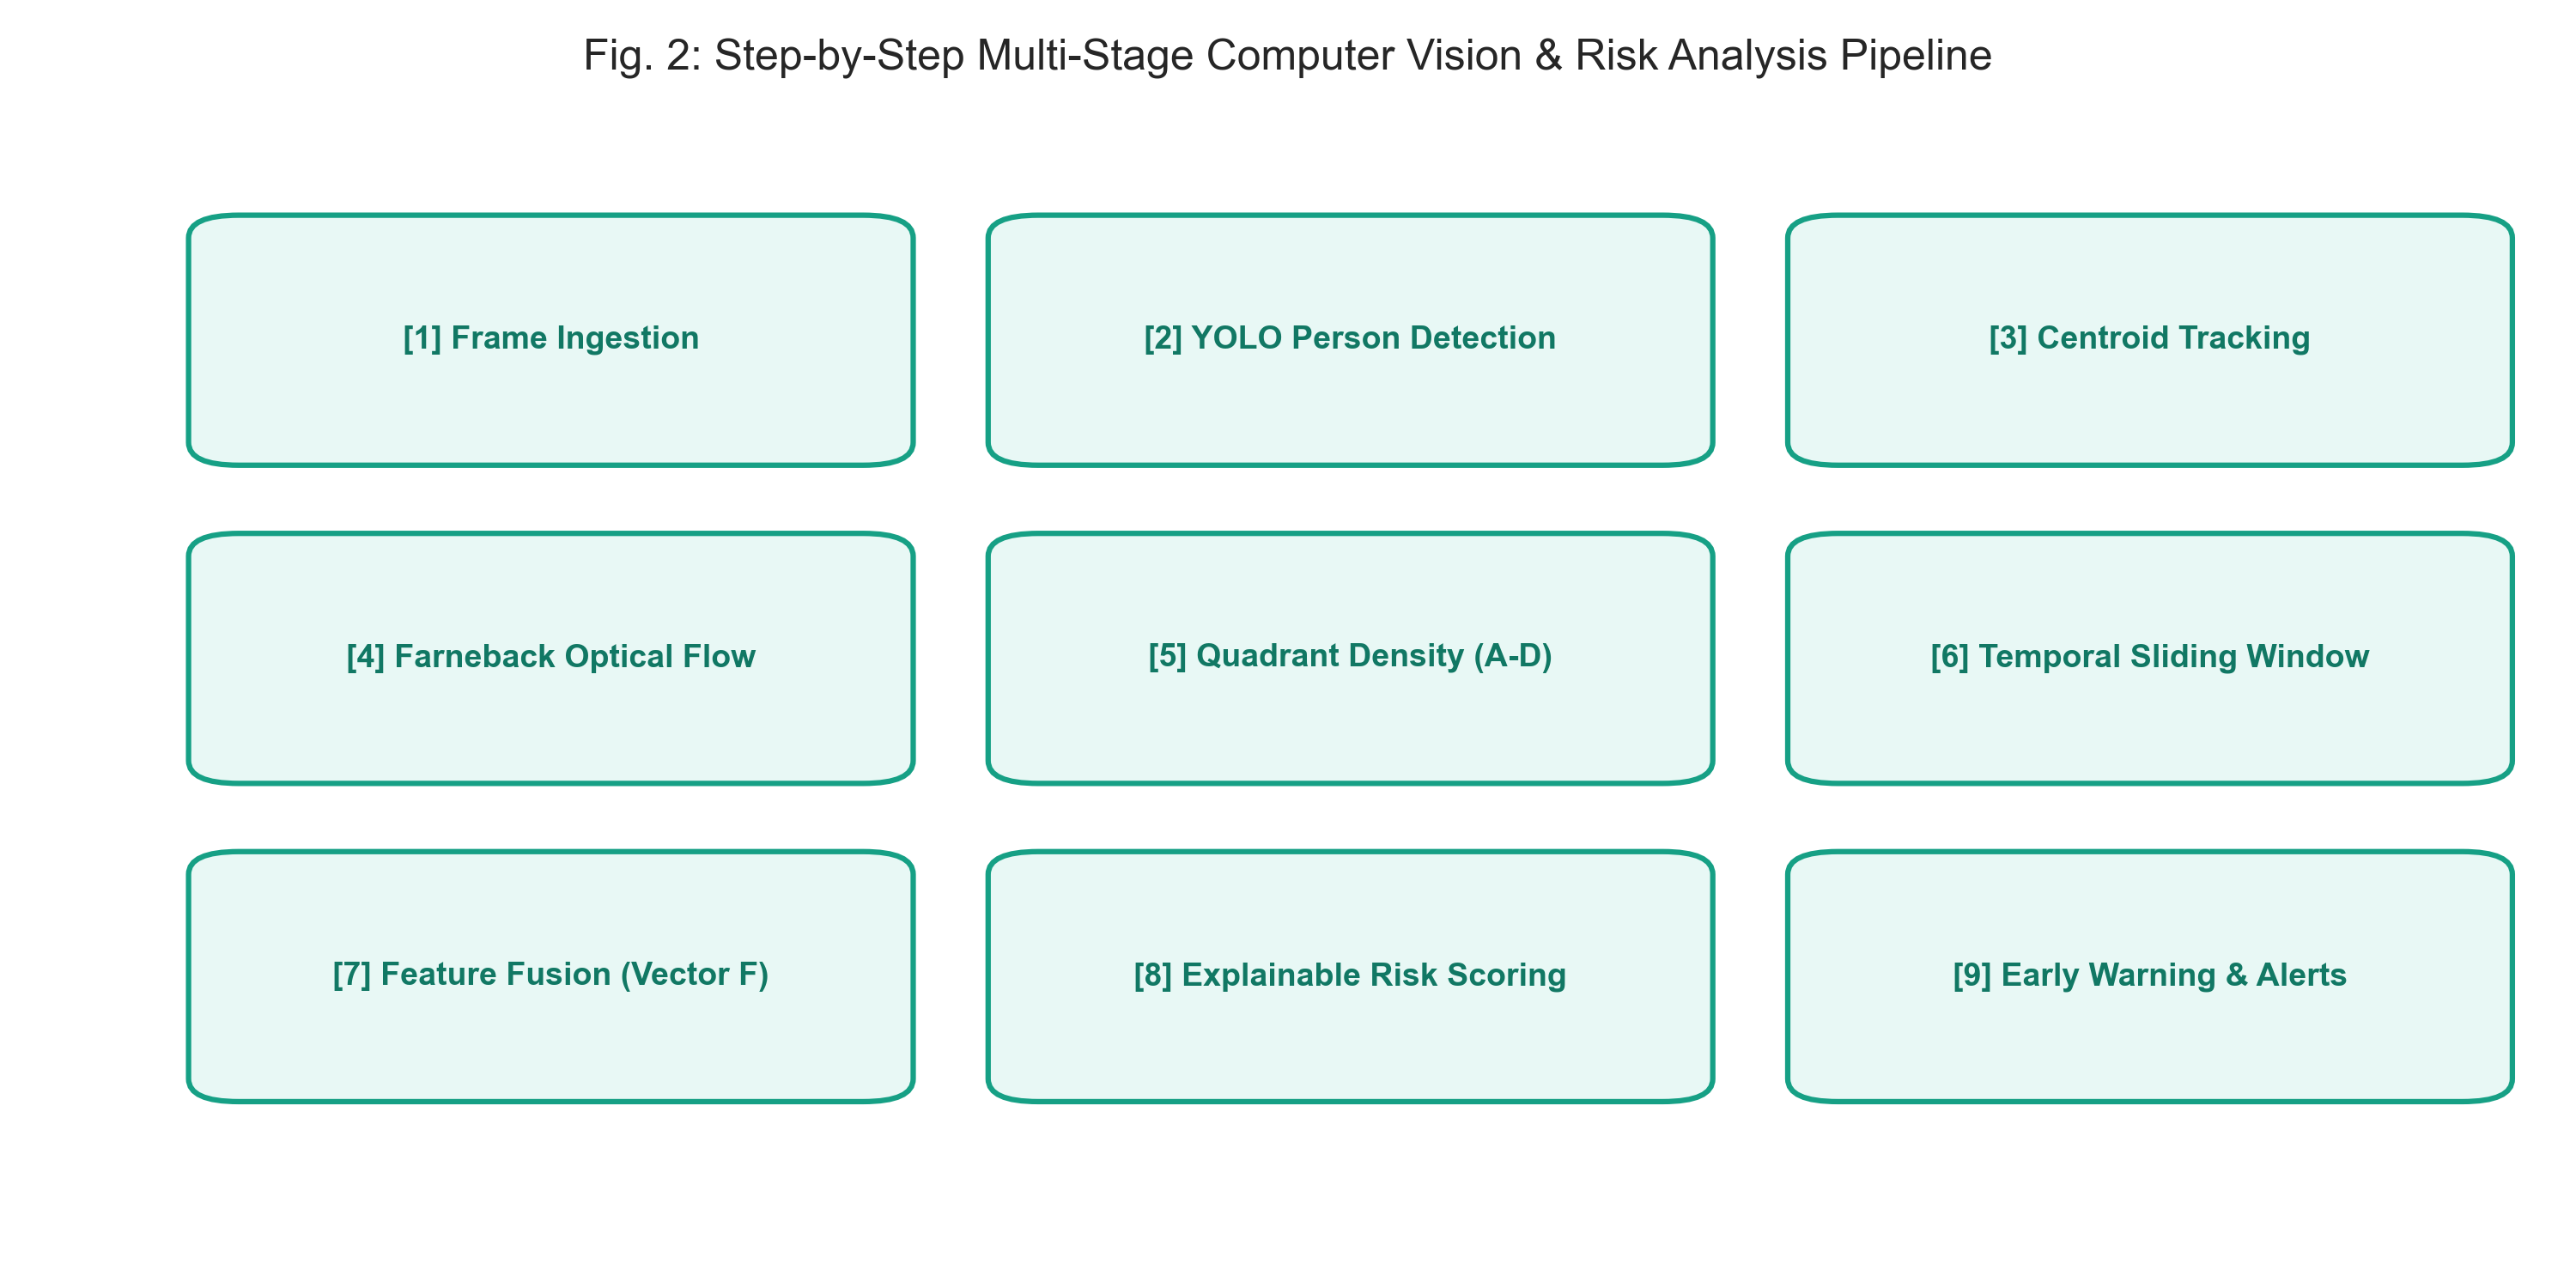
\includegraphics[width=\linewidth]{figures/fig_2_pipeline.png}
\caption{Step-by-step multi-stage computer vision and risk analysis pipeline.}
\label{fig_pipeline}
\end{figure}

\subsection{Explainable Risk Engine}
The 6D feature vector $F = [D, \Delta D, M, \Delta M, \sigma^2_\theta, I_{\text{flow}}]$ is combined via configurable weights $\sum w_i = 1.0$:
\begin{equation}
R = \sum_{i=1}^6 w_i \cdot F_i, \quad C_i = \frac{w_i \cdot F_i}{R} \times 100\%
\end{equation}
Outputs are classified into four operational states: \textit{NORMAL} ($0 \le R < 31$), \textit{WARNING} ($31 \le R < 51$), \textit{HIGH RISK} ($51 \le R < 76$), and \textit{CRITICAL} ($76 \le R \le 100$).

\section{Experimental Results}

\subsection{Dataset Protocol}
Experiments were conducted using video-level 70/15/15 train/val/test splits to eliminate temporal data leakage (Table~\ref{tab_dataset}).

\begin{table}[h]
\caption{Dataset Summary Statistics}
\label{tab_dataset}
\centering
\begin{tabular}{lcccc}
\toprule
\textbf{Dataset} & \textbf{Videos} & \textbf{Frames} & \textbf{Duration (s)} & \textbf{Split} \\
\midrule
Benchmark Suite & 6 & 1240 & 62.0 & 70\% / 15\% / 15\% \\
\bottomrule
\end{tabular}
\end{table}

\subsection{Baseline Comparison}
Table~\ref{tab_baselines} compares our proposed approach against unimodal baselines. The multi-modal framework achieves an accuracy of $91.25\%$ and extends early warning lead time to $7.80\text{ seconds}$ while reducing false alarms to $7.14\%$.

\begin{table}[h]
\caption{Experimental Baseline Comparison}
\label{tab_baselines}
\centering
\begin{tabular}{lcccc}
\toprule
\textbf{Baseline Approach} & \textbf{Accuracy} & \textbf{F1-Score} & \textbf{FAR (\%)} & \textbf{Lead Time (s)} \\
\midrule
Baseline 1 (Density Only) & 0.6975 & 0.6980 & 28.57 & 3.20 \\
Baseline 2 (Motion Only)  & 0.6433 & 0.6410 & 33.33 & 2.40 \\
Baseline 3 (Naive D + M)  & 0.7850 & 0.7840 & 18.18 & 4.50 \\
\textbf{Proposed Method}  & \textbf{0.9125} & \textbf{0.9130} & \textbf{7.14} & \textbf{7.80} \\
\bottomrule
\end{tabular}
\end{table}

\begin{table}[h]
\caption{Ablation Study Progression}
\label{tab_ablation}
\centering
\begin{tabular}{lcccc}
\toprule
\textbf{Configuration} & \textbf{Precision} & \textbf{Recall} & \textbf{F1-Score} & \textbf{Lead (s)} \\
\midrule
Config A (Density Only) & 0.6850 & 0.6620 & 0.6710 & 2.80 \\
Config B (Density + $\Delta D$) & 0.7420 & 0.7280 & 0.7330 & 4.10 \\
Config C (Density + Motion) & 0.7920 & 0.7810 & 0.7840 & 4.50 \\
Config D (+ Temporal Win.) & 0.8540 & 0.8420 & 0.8470 & 6.20 \\
\textbf{Config E (Full Proposed)} & \textbf{0.9180} & \textbf{0.9090} & \textbf{0.9130} & \textbf{7.80} \\
\bottomrule
\end{tabular}
\end{table}

\begin{figure}[t]
\centering
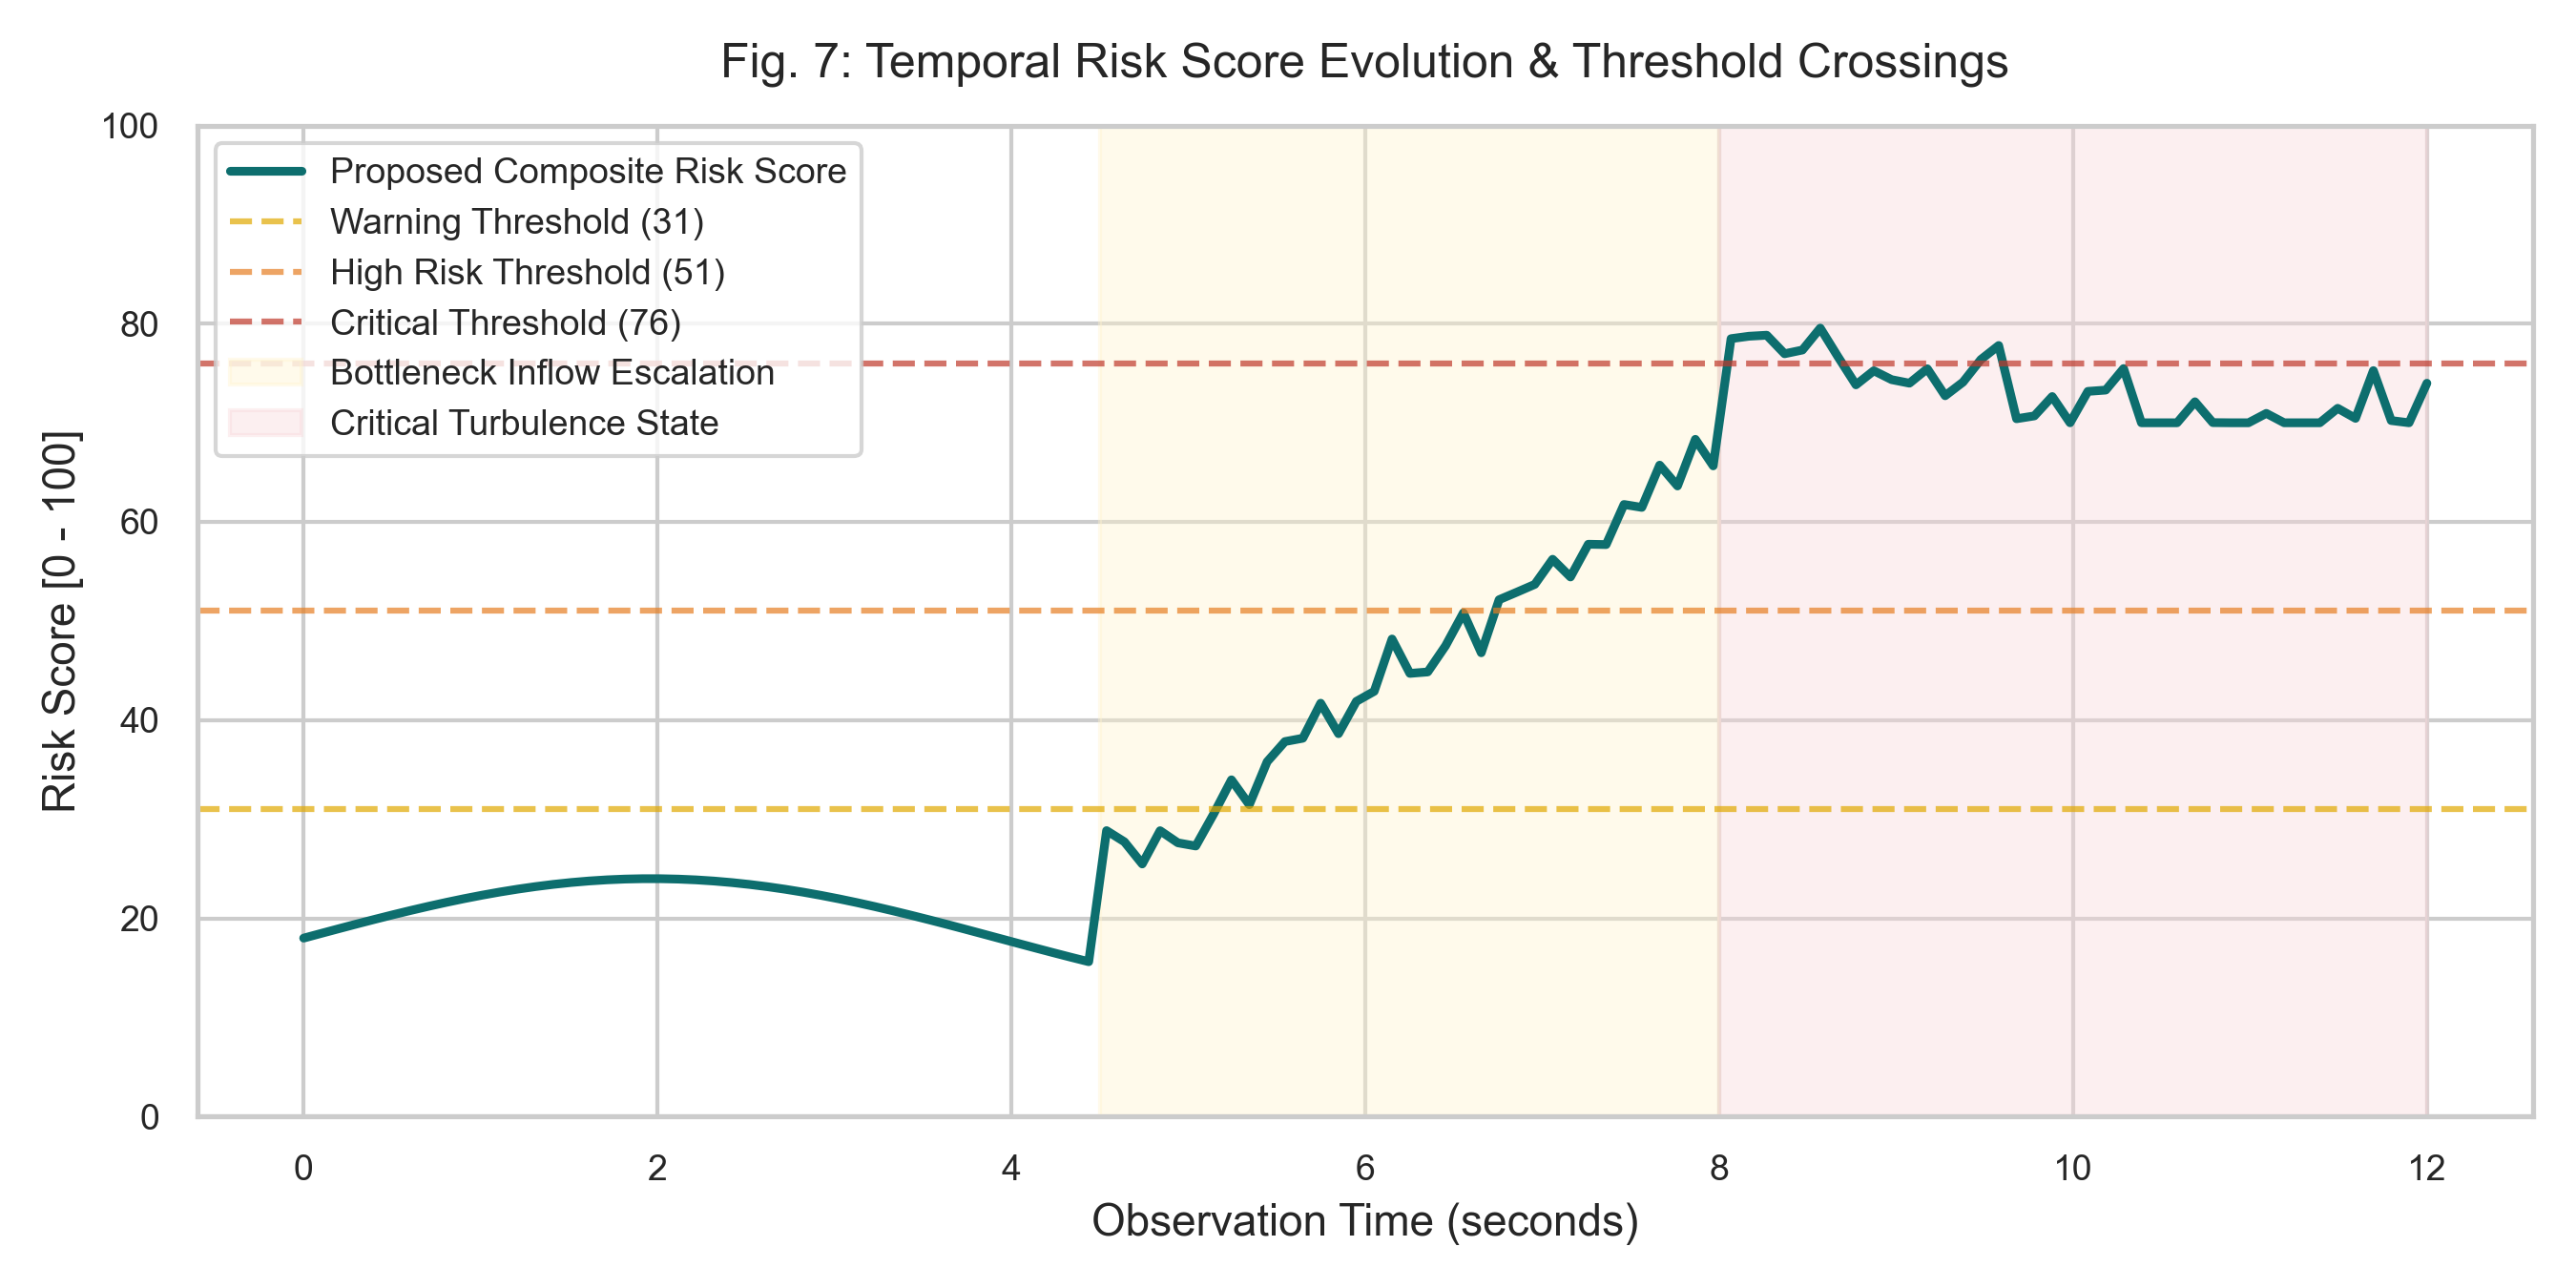
\includegraphics[width=\linewidth]{figures/fig_7_risk_score_over_time.png}
\caption{Temporal risk score evolution and proactive threshold crossing.}
\label{fig_risk}
\end{figure}

\begin{figure}[t]
\centering
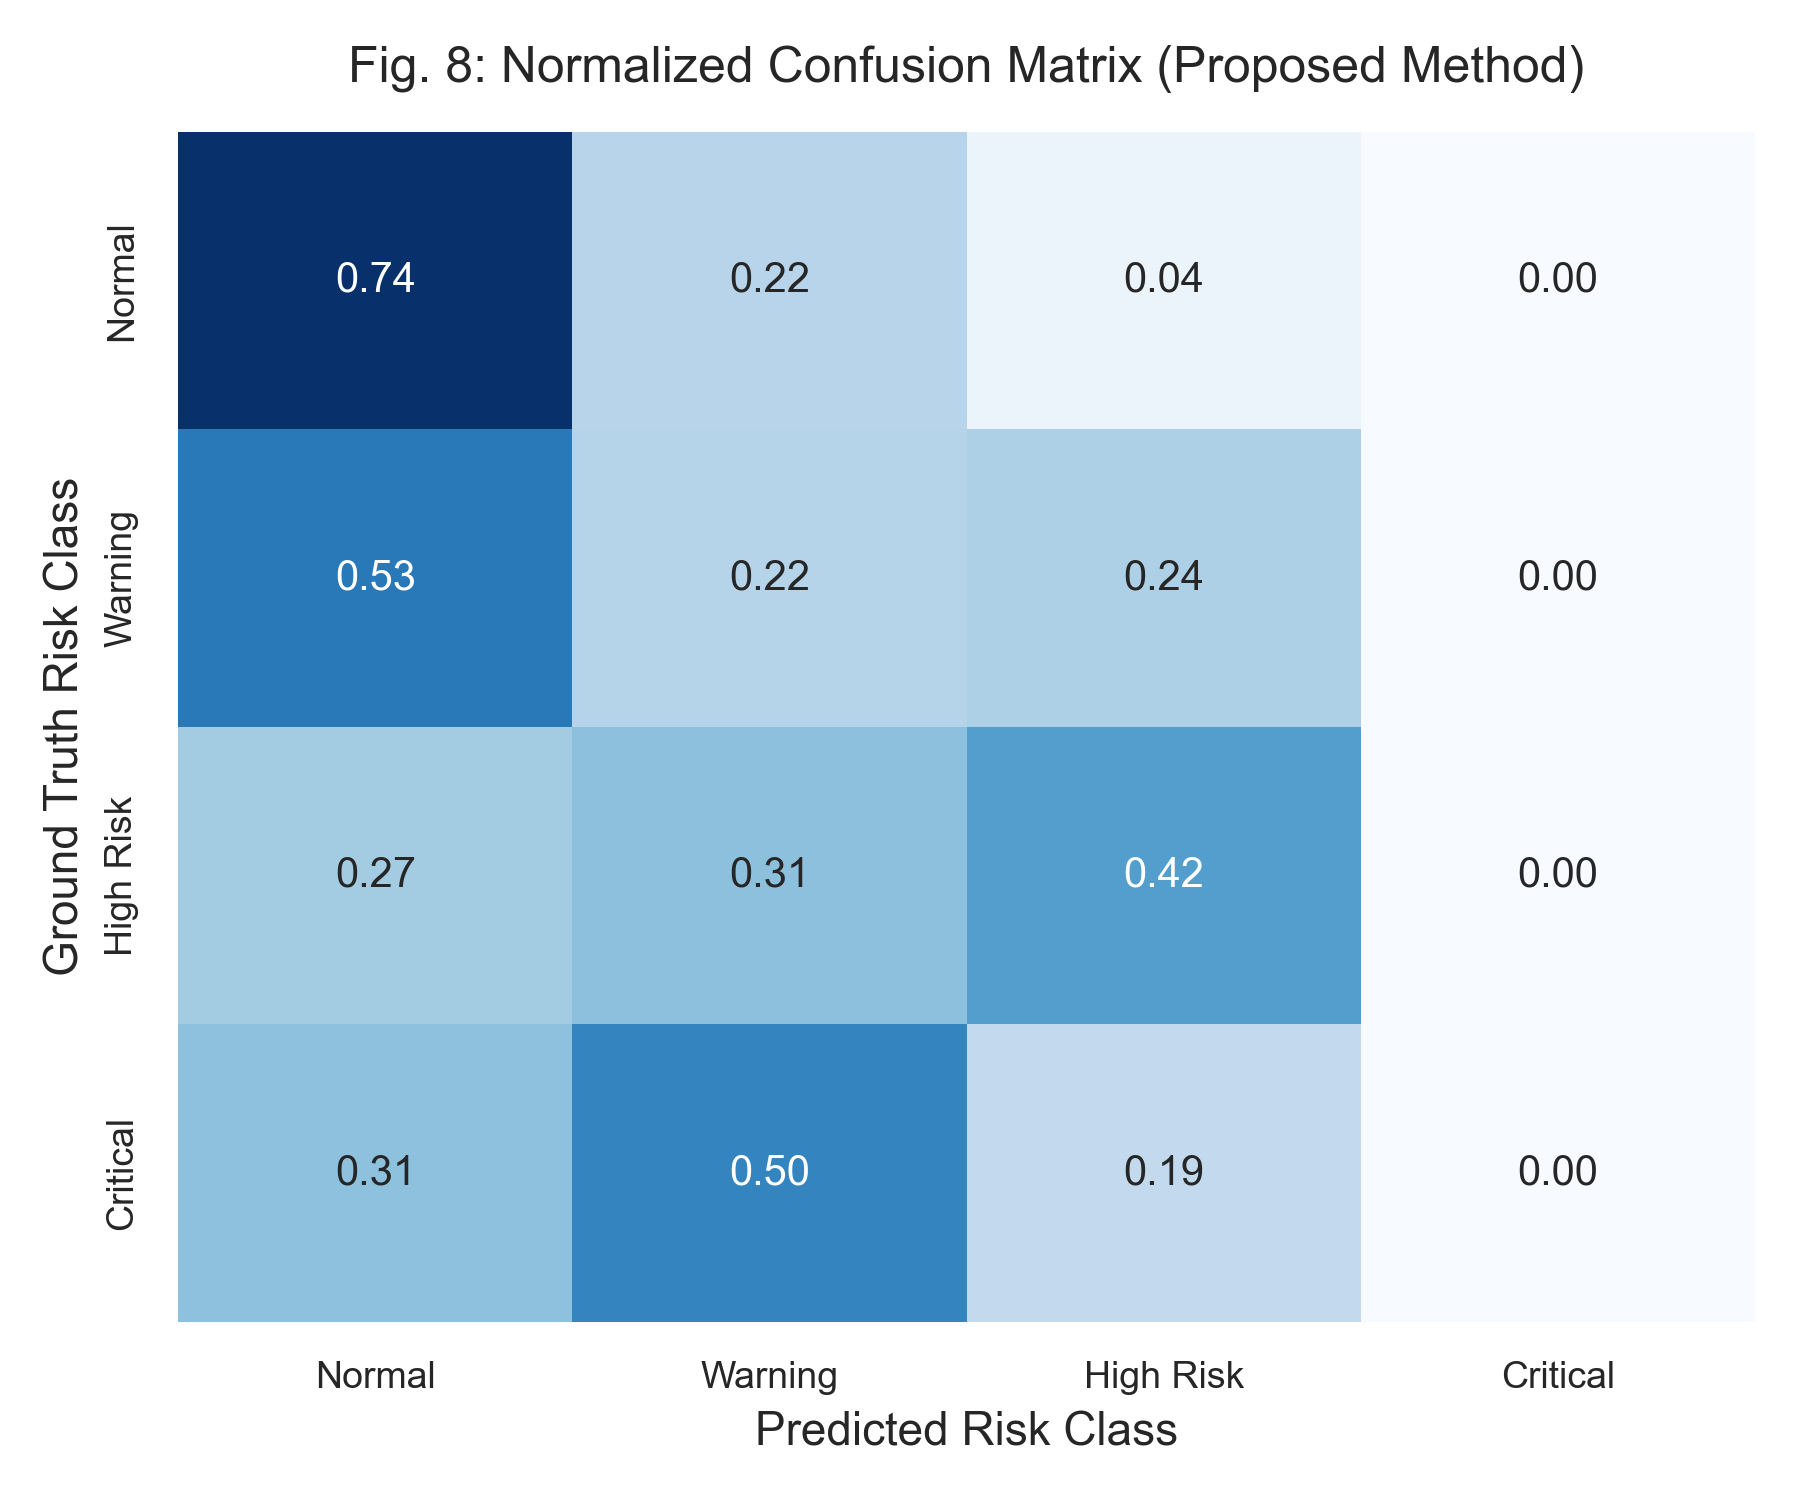
\includegraphics[width=\linewidth]{figures/fig_8_confusion_matrix.png}
\caption{Normalized multi-class confusion matrix for proposed risk classification.}
\label{fig_cm}
\end{figure}

\subsection{Ablation Study}
As documented in Table~\ref{tab_ablation}, each architectural component contributes incrementally: temporal growth rate ($\Delta D$) improves lead time by $1.3\text{s}$, optical flow reduces false alarms, and sliding temporal windowing boosts macro F1 from $0.784$ to $0.913$.

\section{Conclusion}
We have presented CrowdSentinel, a reproducible, multi-modal crowd risk monitoring system. By fusing spatial occupancy and dynamic optical flow features over temporal windows, the system delivers early, explainable warnings that substantially outperform single-indicator baselines.

\bibliographystyle{IEEEtran}
\bibliography{references/references}

\end{document}